\documentclass{standalone}
\usepackage{tikz}
\usetikzlibrary{patterns, positioning}


\begin{document}
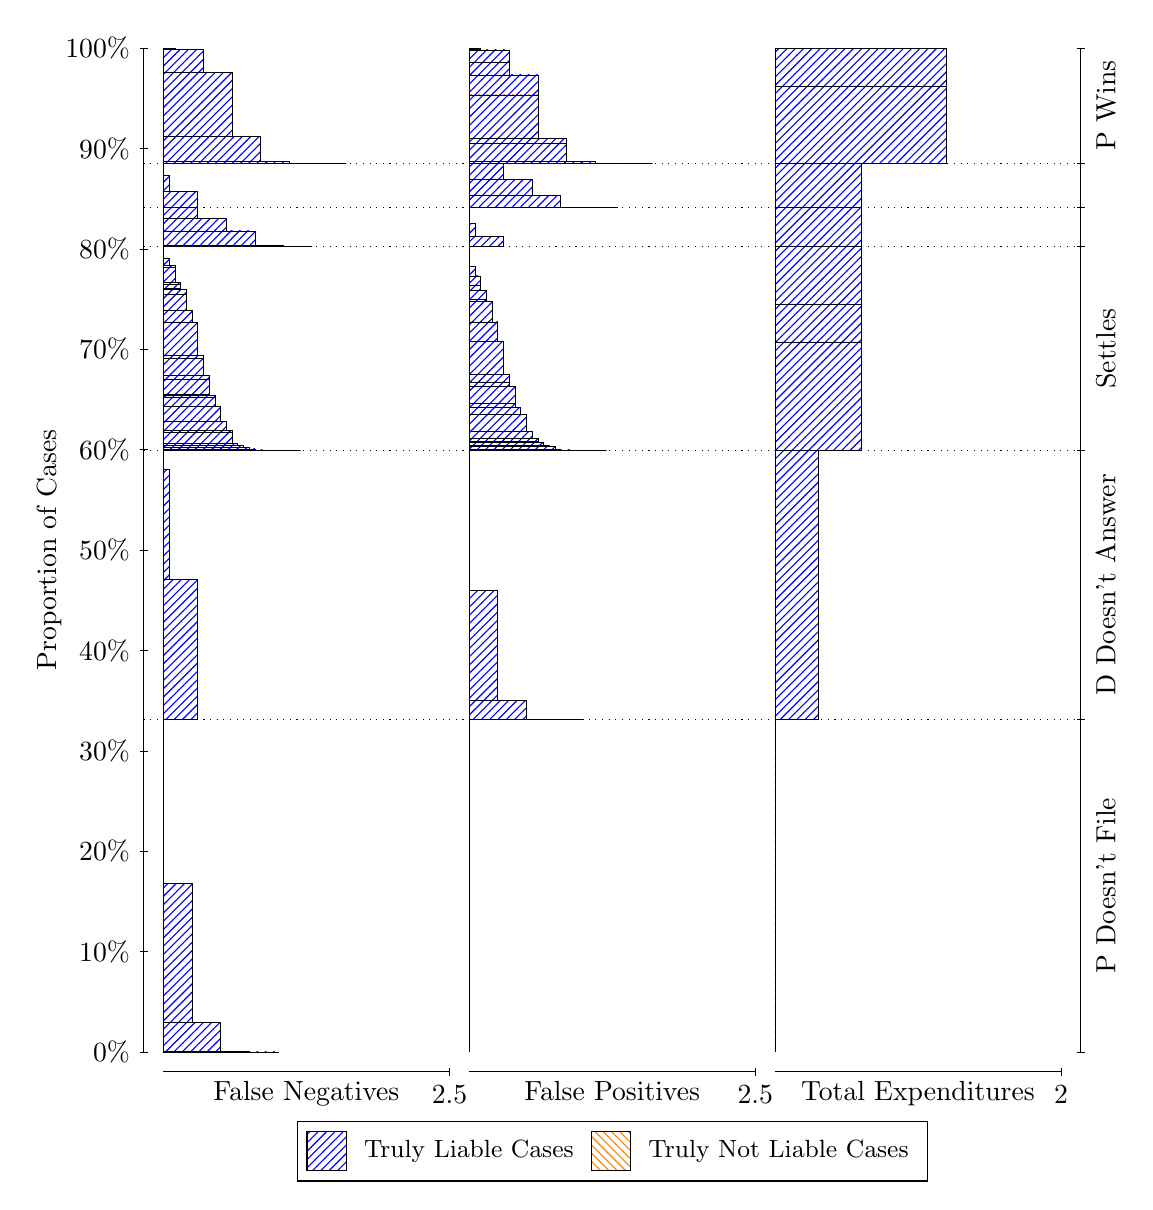
\begin{tikzpicture}
\draw[black, very thin] (1.5,1.75) -- (1.5,14.5);
\node[rotate=90, text=black, anchor=center] at (0.3, 8.125) {Proportion of Cases};
\draw[black, very thin] (1.45,1.75) -- (1.55,1.75);
\node[text=black, anchor=east] at (1.45, 1.75) {0\%};
\draw[black, very thin] (1.45,3.025) -- (1.55,3.025);
\node[text=black, anchor=east] at (1.45, 3.025) {10\%};
\draw[black, very thin] (1.45,4.3) -- (1.55,4.3);
\node[text=black, anchor=east] at (1.45, 4.3) {20\%};
\draw[black, very thin] (1.45,5.575) -- (1.55,5.575);
\node[text=black, anchor=east] at (1.45, 5.575) {30\%};
\draw[black, very thin] (1.45,6.85) -- (1.55,6.85);
\node[text=black, anchor=east] at (1.45, 6.85) {40\%};
\draw[black, very thin] (1.45,8.125) -- (1.55,8.125);
\node[text=black, anchor=east] at (1.45, 8.125) {50\%};
\draw[black, very thin] (1.45,9.4) -- (1.55,9.4);
\node[text=black, anchor=east] at (1.45, 9.4) {60\%};
\draw[black, very thin] (1.45,10.675) -- (1.55,10.675);
\node[text=black, anchor=east] at (1.45, 10.675) {70\%};
\draw[black, very thin] (1.45,11.95) -- (1.55,11.95);
\node[text=black, anchor=east] at (1.45, 11.95) {80\%};
\draw[black, very thin] (1.45,13.225) -- (1.55,13.225);
\node[text=black, anchor=east] at (1.45, 13.225) {90\%};
\draw[black, very thin] (1.45,14.5) -- (1.55,14.5);
\node[text=black, anchor=east] at (1.45, 14.5) {100\%};

\draw[black, very thin] (13.4,1.75) -- (13.4,14.5);
\draw[black, very thin] (13.35,1.75) -- (13.45,1.75);
\node[anchor=west] at (13.35, 1.75) {};
\draw[black, very thin] (13.35,5.9716) -- (13.45,5.9716);
\node[anchor=west] at (13.35, 5.9716) {};
\draw[black, very thin] (13.35,9.3909) -- (13.45,9.3909);
\node[anchor=west] at (13.35, 9.3909) {};
\draw[black, very thin] (13.35,11.976) -- (13.45,11.976);
\node[anchor=west] at (13.35, 11.976) {};
\draw[black, very thin] (13.35,12.472) -- (13.45,12.472);
\node[anchor=west] at (13.35, 12.472) {};
\draw[black, very thin] (13.35,13.037) -- (13.45,13.037);
\node[anchor=west] at (13.35, 13.037) {};
\draw[black, very thin] (13.35,14.5) -- (13.45,14.5);
\node[anchor=west] at (13.35, 14.5) {};

\draw[black, very thin, pattern color=blue, pattern=north east lines] (1.75,1.75) rectangle (3.2033,1.7501);
\draw[black, very thin, pattern color=blue, pattern=north east lines] (1.75,1.7501) rectangle (2.84,1.761);
\draw[black, very thin, pattern color=blue, pattern=north east lines] (1.75,1.761) rectangle (2.4767,2.1269);
\draw[black, very thin, pattern color=blue, pattern=north east lines] (1.75,2.1269) rectangle (2.1133,3.8893);
\draw[black, very thin, pattern color=orange, pattern=north west lines] (1.75,3.8893) rectangle (1.75,3.8893);
\draw[black, very thin, pattern color=blue, pattern=north east lines] (1.75,3.8893) rectangle (1.75,5.9716);
\draw[black, very thin, pattern color=blue, pattern=north east lines] (1.75,5.9716) rectangle (2.186,7.7531);
\draw[black, very thin, pattern color=blue, pattern=north east lines] (1.75,7.7531) rectangle (1.8227,9.1494);
\draw[black, very thin, pattern color=orange, pattern=north west lines] (1.75,9.1494) rectangle (1.75,9.1494);
\draw[black, very thin, pattern color=blue, pattern=north east lines] (1.75,9.1494) rectangle (1.75,9.3909);
\draw[black, very thin, pattern color=blue, pattern=north east lines] (1.75,9.3909) rectangle (3.494,9.3909);
\draw[black, very thin, pattern color=blue, pattern=north east lines] (1.75,9.3909) rectangle (3.3487,9.3909);
\draw[black, very thin, pattern color=blue, pattern=north east lines] (1.75,9.3909) rectangle (3.2033,9.3929);
\draw[black, very thin, pattern color=blue, pattern=north east lines] (1.75,9.3929) rectangle (3.1307,9.3938);
\draw[black, very thin, pattern color=blue, pattern=north east lines] (1.75,9.3938) rectangle (3.058,9.3938);
\draw[black, very thin, pattern color=blue, pattern=north east lines] (1.75,9.3938) rectangle (3.058,9.3959);
\draw[black, very thin, pattern color=blue, pattern=north east lines] (1.75,9.3959) rectangle (2.9853,9.3971);
\draw[black, very thin, pattern color=blue, pattern=north east lines] (1.75,9.3971) rectangle (2.9127,9.4085);
\draw[black, very thin, pattern color=blue, pattern=north east lines] (1.75,9.4085) rectangle (2.84,9.4278);
\draw[black, very thin, pattern color=blue, pattern=north east lines] (1.75,9.4278) rectangle (2.7673,9.4512);
\draw[black, very thin, pattern color=blue, pattern=north east lines] (1.75,9.4512) rectangle (2.6947,9.454);
\draw[black, very thin, pattern color=blue, pattern=north east lines] (1.75,9.454) rectangle (2.6947,9.4837);
\draw[black, very thin, pattern color=blue, pattern=north east lines] (1.75,9.4837) rectangle (2.622,9.6248);
\draw[black, very thin, pattern color=blue, pattern=north east lines] (1.75,9.6248) rectangle (2.622,9.6404);
\draw[black, very thin, pattern color=blue, pattern=north east lines] (1.75,9.6404) rectangle (2.5493,9.7609);
\draw[black, very thin, pattern color=blue, pattern=north east lines] (1.75,9.7609) rectangle (2.4767,9.9442);
\draw[black, very thin, pattern color=blue, pattern=north east lines] (1.75,9.9442) rectangle (2.404,10.063);
\draw[black, very thin, pattern color=blue, pattern=north east lines] (1.75,10.063) rectangle (2.404,10.085);
\draw[black, very thin, pattern color=blue, pattern=north east lines] (1.75,10.085) rectangle (2.3313,10.107);
\draw[black, very thin, pattern color=blue, pattern=north east lines] (1.75,10.107) rectangle (2.3313,10.292);
\draw[black, very thin, pattern color=blue, pattern=north east lines] (1.75,10.292) rectangle (2.3313,10.344);
\draw[black, very thin, pattern color=blue, pattern=north east lines] (1.75,10.344) rectangle (2.2587,10.565);
\draw[black, very thin, pattern color=blue, pattern=north east lines] (1.75,10.565) rectangle (2.2587,10.596);
\draw[black, very thin, pattern color=blue, pattern=north east lines] (1.75,10.596) rectangle (2.186,11.012);
\draw[black, very thin, pattern color=blue, pattern=north east lines] (1.75,11.012) rectangle (2.1133,11.164);
\draw[black, very thin, pattern color=blue, pattern=north east lines] (1.75,11.164) rectangle (2.0407,11.375);
\draw[black, very thin, pattern color=blue, pattern=north east lines] (1.75,11.375) rectangle (2.0407,11.433);
\draw[black, very thin, pattern color=blue, pattern=north east lines] (1.75,11.433) rectangle (1.968,11.448);
\draw[black, very thin, pattern color=blue, pattern=north east lines] (1.75,11.448) rectangle (1.968,11.498);
\draw[black, very thin, pattern color=blue, pattern=north east lines] (1.75,11.498) rectangle (1.968,11.519);
\draw[black, very thin, pattern color=blue, pattern=north east lines] (1.75,11.519) rectangle (1.8953,11.72);
\draw[black, very thin, pattern color=blue, pattern=north east lines] (1.75,11.72) rectangle (1.8953,11.74);
\draw[black, very thin, pattern color=blue, pattern=north east lines] (1.75,11.74) rectangle (1.8227,11.828);
\draw[black, very thin, pattern color=orange, pattern=north west lines] (1.75,11.828) rectangle (1.75,11.828);
\draw[black, very thin, pattern color=blue, pattern=north east lines] (1.75,11.828) rectangle (1.75,11.976);
\draw[black, very thin, pattern color=blue, pattern=north east lines] (1.75,11.976) rectangle (3.6393,11.976);
\draw[black, very thin, pattern color=blue, pattern=north east lines] (1.75,11.976) rectangle (3.276,11.993);
\draw[black, very thin, pattern color=blue, pattern=north east lines] (1.75,11.993) rectangle (2.9127,12.179);
\draw[black, very thin, pattern color=blue, pattern=north east lines] (1.75,12.179) rectangle (2.5493,12.338);
\draw[black, very thin, pattern color=blue, pattern=north east lines] (1.75,12.338) rectangle (2.186,12.472);
\draw[black, very thin, pattern color=orange, pattern=north west lines] (1.75,12.472) rectangle (1.75,12.472);
\draw[black, very thin, pattern color=blue, pattern=north east lines] (1.75,12.472) rectangle (2.186,12.68);
\draw[black, very thin, pattern color=blue, pattern=north east lines] (1.75,12.68) rectangle (1.8227,12.879);
\draw[black, very thin, pattern color=orange, pattern=north west lines] (1.75,12.879) rectangle (1.75,12.879);
\draw[black, very thin, pattern color=blue, pattern=north east lines] (1.75,12.879) rectangle (1.75,13.037);
\draw[black, very thin, pattern color=blue, pattern=north east lines] (1.75,13.037) rectangle (4.0753,13.037);
\draw[black, very thin, pattern color=blue, pattern=north east lines] (1.75,13.037) rectangle (3.712,13.037);
\draw[black, very thin, pattern color=blue, pattern=north east lines] (1.75,13.037) rectangle (3.3487,13.062);
\draw[black, very thin, pattern color=blue, pattern=north east lines] (1.75,13.062) rectangle (2.9853,13.377);
\draw[black, very thin, pattern color=blue, pattern=north east lines] (1.75,13.377) rectangle (2.622,14.187);
\draw[black, very thin, pattern color=blue, pattern=north east lines] (1.75,14.187) rectangle (2.2587,14.479);
\draw[black, very thin, pattern color=blue, pattern=north east lines] (1.75,14.479) rectangle (1.8953,14.5);
\draw[black, very thin, pattern color=orange, pattern=north west lines] (1.75,14.5) rectangle (1.75,14.5);
\draw[black, very thin, pattern color=blue, pattern=north east lines] (1.75,14.5) rectangle (1.75,14.5);
\draw[black, very thin, pattern color=orange, pattern=north west lines] (5.6333,1.75) rectangle (5.6333,1.75);
\draw[black, very thin, pattern color=blue, pattern=north east lines] (5.6333,1.75) rectangle (5.6333,5.9716);
\draw[black, very thin, pattern color=orange, pattern=north west lines] (5.6333,5.9716) rectangle (7.0867,5.9716);
\draw[black, very thin, pattern color=blue, pattern=north east lines] (5.6333,5.9716) rectangle (7.0867,5.9716);
\draw[black, very thin, pattern color=blue, pattern=north east lines] (5.6333,5.9716) rectangle (6.7233,5.9738);
\draw[black, very thin, pattern color=blue, pattern=north east lines] (5.6333,5.9738) rectangle (6.36,6.213);
\draw[black, very thin, pattern color=blue, pattern=north east lines] (5.6333,6.213) rectangle (5.9967,7.6093);
\draw[black, very thin, pattern color=blue, pattern=north east lines] (5.6333,7.6093) rectangle (5.6333,9.3909);
\draw[black, very thin, pattern color=orange, pattern=north west lines] (5.6333,9.3909) rectangle (7.3773,9.3909);
\draw[black, very thin, pattern color=blue, pattern=north east lines] (5.6333,9.3909) rectangle (7.3773,9.3909);
\draw[black, very thin, pattern color=orange, pattern=north west lines] (5.6333,9.3909) rectangle (7.232,9.3909);
\draw[black, very thin, pattern color=blue, pattern=north east lines] (5.6333,9.3909) rectangle (7.232,9.3909);
\draw[black, very thin, pattern color=orange, pattern=north west lines] (5.6333,9.3909) rectangle (7.0867,9.3909);
\draw[black, very thin, pattern color=blue, pattern=north east lines] (5.6333,9.3909) rectangle (7.0867,9.3937);
\draw[black, very thin, pattern color=blue, pattern=north east lines] (5.6333,9.3937) rectangle (7.014,9.394);
\draw[black, very thin, pattern color=orange, pattern=north west lines] (5.6333,9.394) rectangle (6.9413,9.394);
\draw[black, very thin, pattern color=blue, pattern=north east lines] (5.6333,9.394) rectangle (6.9413,9.3968);
\draw[black, very thin, pattern color=blue, pattern=north east lines] (5.6333,9.3968) rectangle (6.8687,9.3974);
\draw[black, very thin, pattern color=orange, pattern=north west lines] (5.6333,9.3974) rectangle (6.796,9.3974);
\draw[black, very thin, pattern color=blue, pattern=north east lines] (5.6333,9.3974) rectangle (6.796,9.4056);
\draw[black, very thin, pattern color=blue, pattern=north east lines] (5.6333,9.4056) rectangle (6.7233,9.4382);
\draw[black, very thin, pattern color=orange, pattern=north west lines] (5.6333,9.4382) rectangle (6.6507,9.4382);
\draw[black, very thin, pattern color=blue, pattern=north east lines] (5.6333,9.4382) rectangle (6.6507,9.4489);
\draw[black, very thin, pattern color=blue, pattern=north east lines] (5.6333,9.4489) rectangle (6.578,9.4869);
\draw[black, very thin, pattern color=blue, pattern=north east lines] (5.6333,9.4869) rectangle (6.5053,9.5028);
\draw[black, very thin, pattern color=orange, pattern=north west lines] (5.6333,9.5028) rectangle (6.5053,9.5028);
\draw[black, very thin, pattern color=blue, pattern=north east lines] (5.6333,9.5028) rectangle (6.5053,9.5388);
\draw[black, very thin, pattern color=blue, pattern=north east lines] (5.6333,9.5388) rectangle (6.4327,9.6267);
\draw[black, very thin, pattern color=orange, pattern=north west lines] (5.6333,9.6267) rectangle (6.36,9.6267);
\draw[black, very thin, pattern color=blue, pattern=north east lines] (5.6333,9.6267) rectangle (6.36,9.8482);
\draw[black, very thin, pattern color=blue, pattern=north east lines] (5.6333,9.8482) rectangle (6.2873,9.9337);
\draw[black, very thin, pattern color=orange, pattern=north west lines] (5.6333,9.9337) rectangle (6.2147,9.9337);
\draw[black, very thin, pattern color=blue, pattern=north east lines] (5.6333,9.9337) rectangle (6.2147,9.9915);
\draw[black, very thin, pattern color=blue, pattern=north east lines] (5.6333,9.9915) rectangle (6.2147,10.203);
\draw[black, very thin, pattern color=blue, pattern=north east lines] (5.6333,10.203) rectangle (6.142,10.26);
\draw[black, very thin, pattern color=blue, pattern=north east lines] (5.6333,10.26) rectangle (6.142,10.355);
\draw[black, very thin, pattern color=blue, pattern=north east lines] (5.6333,10.355) rectangle (6.0693,10.771);
\draw[black, very thin, pattern color=blue, pattern=north east lines] (5.6333,10.771) rectangle (5.9967,11.023);
\draw[black, very thin, pattern color=blue, pattern=north east lines] (5.6333,11.023) rectangle (5.924,11.282);
\draw[black, very thin, pattern color=blue, pattern=north east lines] (5.6333,11.282) rectangle (5.8513,11.304);
\draw[black, very thin, pattern color=blue, pattern=north east lines] (5.6333,11.304) rectangle (5.8513,11.423);
\draw[black, very thin, pattern color=blue, pattern=north east lines] (5.6333,11.423) rectangle (5.7787,11.484);
\draw[black, very thin, pattern color=blue, pattern=north east lines] (5.6333,11.484) rectangle (5.7787,11.606);
\draw[black, very thin, pattern color=blue, pattern=north east lines] (5.6333,11.606) rectangle (5.706,11.726);
\draw[black, very thin, pattern color=blue, pattern=north east lines] (5.6333,11.726) rectangle (5.6333,11.976);
\draw[black, very thin, pattern color=orange, pattern=north west lines] (5.6333,11.976) rectangle (6.0693,11.976);
\draw[black, very thin, pattern color=blue, pattern=north east lines] (5.6333,11.976) rectangle (6.0693,12.11);
\draw[black, very thin, pattern color=blue, pattern=north east lines] (5.6333,12.11) rectangle (5.706,12.269);
\draw[black, very thin, pattern color=blue, pattern=north east lines] (5.6333,12.269) rectangle (5.6333,12.472);
\draw[black, very thin, pattern color=orange, pattern=north west lines] (5.6333,12.472) rectangle (7.5227,12.472);
\draw[black, very thin, pattern color=blue, pattern=north east lines] (5.6333,12.472) rectangle (7.5227,12.472);
\draw[black, very thin, pattern color=blue, pattern=north east lines] (5.6333,12.472) rectangle (7.1593,12.481);
\draw[black, very thin, pattern color=blue, pattern=north east lines] (5.6333,12.481) rectangle (6.796,12.629);
\draw[black, very thin, pattern color=blue, pattern=north east lines] (5.6333,12.629) rectangle (6.4327,12.828);
\draw[black, very thin, pattern color=blue, pattern=north east lines] (5.6333,12.828) rectangle (6.0693,13.037);
\draw[black, very thin, pattern color=orange, pattern=north west lines] (5.6333,13.037) rectangle (7.9587,13.037);
\draw[black, very thin, pattern color=blue, pattern=north east lines] (5.6333,13.037) rectangle (7.9587,13.037);
\draw[black, very thin, pattern color=orange, pattern=north west lines] (5.6333,13.037) rectangle (7.5953,13.037);
\draw[black, very thin, pattern color=blue, pattern=north east lines] (5.6333,13.037) rectangle (7.5953,13.037);
\draw[black, very thin, pattern color=orange, pattern=north west lines] (5.6333,13.037) rectangle (7.232,13.037);
\draw[black, very thin, pattern color=blue, pattern=north east lines] (5.6333,13.037) rectangle (7.232,13.058);
\draw[black, very thin, pattern color=blue, pattern=north east lines] (5.6333,13.058) rectangle (6.8687,13.289);
\draw[black, very thin, pattern color=orange, pattern=north west lines] (5.6333,13.289) rectangle (6.8687,13.289);
\draw[black, very thin, pattern color=blue, pattern=north east lines] (5.6333,13.289) rectangle (6.8687,13.35);
\draw[black, very thin, pattern color=blue, pattern=north east lines] (5.6333,13.35) rectangle (6.5053,13.905);
\draw[black, very thin, pattern color=orange, pattern=north west lines] (5.6333,13.905) rectangle (6.5053,13.905);
\draw[black, very thin, pattern color=blue, pattern=north east lines] (5.6333,13.905) rectangle (6.5053,14.159);
\draw[black, very thin, pattern color=blue, pattern=north east lines] (5.6333,14.159) rectangle (6.142,14.322);
\draw[black, very thin, pattern color=blue, pattern=north east lines] (5.6333,14.322) rectangle (6.142,14.475);
\draw[black, very thin, pattern color=blue, pattern=north east lines] (5.6333,14.475) rectangle (5.7787,14.483);
\draw[black, very thin, pattern color=blue, pattern=north east lines] (5.6333,14.483) rectangle (5.7787,14.5);
\draw[black, very thin, pattern color=blue, pattern=north east lines] (5.6333,14.5) rectangle (5.6333,14.5);
\draw[black, very thin, pattern color=orange, pattern=north west lines] (9.5167,1.75) rectangle (9.5167,1.75);
\draw[black, very thin, pattern color=blue, pattern=north east lines] (9.5167,1.75) rectangle (9.5167,5.9716);
\draw[black, very thin, pattern color=orange, pattern=north west lines] (9.5167,5.9716) rectangle (10.062,5.9716);
\draw[black, very thin, pattern color=blue, pattern=north east lines] (9.5167,5.9716) rectangle (10.062,9.3909);
\draw[black, very thin, pattern color=orange, pattern=north west lines] (9.5167,9.3909) rectangle (10.607,9.3909);
\draw[black, very thin, pattern color=blue, pattern=north east lines] (9.5167,9.3909) rectangle (10.607,10.768);
\draw[black, very thin, pattern color=orange, pattern=north west lines] (9.5167,10.768) rectangle (10.607,10.768);
\draw[black, very thin, pattern color=blue, pattern=north east lines] (9.5167,10.768) rectangle (10.607,11.241);
\draw[black, very thin, pattern color=orange, pattern=north west lines] (9.5167,11.241) rectangle (10.607,11.241);
\draw[black, very thin, pattern color=blue, pattern=north east lines] (9.5167,11.241) rectangle (10.607,11.976);
\draw[black, very thin, pattern color=orange, pattern=north west lines] (9.5167,11.976) rectangle (10.607,11.976);
\draw[black, very thin, pattern color=blue, pattern=north east lines] (9.5167,11.976) rectangle (10.607,12.472);
\draw[black, very thin, pattern color=orange, pattern=north west lines] (9.5167,12.472) rectangle (10.607,12.472);
\draw[black, very thin, pattern color=blue, pattern=north east lines] (9.5167,12.472) rectangle (10.607,13.037);
\draw[black, very thin, pattern color=orange, pattern=north west lines] (9.5167,13.037) rectangle (11.697,13.037);
\draw[black, very thin, pattern color=blue, pattern=north east lines] (9.5167,13.037) rectangle (11.697,14.015);
\draw[black, very thin, pattern color=orange, pattern=north west lines] (9.5167,14.015) rectangle (11.697,14.015);
\draw[black, very thin, pattern color=blue, pattern=north east lines] (9.5167,14.015) rectangle (11.697,14.5);
\draw[black, dotted] (1.5,5.9716) -- (13.4,5.9716);
\draw[black, dotted] (1.5,9.3909) -- (13.4,9.3909);
\draw[black, dotted] (1.5,11.976) -- (13.4,11.976);
\draw[black, dotted] (1.5,12.472) -- (13.4,12.472);
\draw[black, dotted] (1.5,13.037) -- (13.4,13.037);
\draw[black, very thin] (1.75,1.5) -- (5.3833,1.5);
\node[text=black, anchor=north] at (3.5667, 1.5) {False Negatives};
\draw[black, very thin] (5.3833,1.45) -- (5.3833,1.55);
\node[text=black, anchor=north] at (5.3833, 1.45) {2.5};

\draw[black, very thin] (5.6333,1.5) -- (9.2667,1.5);
\node[text=black, anchor=north] at (7.45, 1.5) {False Positives};
\draw[black, very thin] (9.2667,1.45) -- (9.2667,1.55);
\node[text=black, anchor=north] at (9.2667, 1.45) {2.5};

\draw[black, very thin] (9.5167,1.5) -- (13.15,1.5);
\node[text=black, anchor=north] at (11.333, 1.5) {Total Expenditures};
\draw[black, very thin] (13.15,1.45) -- (13.15,1.55);
\node[text=black, anchor=north] at (13.15, 1.45) {2};

\node[text=black, centered, rotate=90] at (13.72, 3.8608) {P Doesn't File};
\node[text=black, centered, rotate=90] at (13.72, 7.6812) {D Doesn't Answer};
\node[text=black, centered, rotate=90] at (13.72, 10.683) {Settles};


\node[text=black, centered, rotate=90] at (13.72, 13.768) {P Wins};

\draw (7.449999999999999,1.5) node[draw=none] (baseCoordinate) {};
\begin{scope}[align=center]
        \matrix[scale=0.5, draw=black, below=0.5cm of baseCoordinate, nodes={draw}, column sep=0.1cm]{
            \node[rectangle, draw, minimum width=0.5cm, minimum height=0.5cm, pattern color=blue, pattern=north east lines] {}; &
            \node[draw=none, font=\small, text=black] (B) {Truly Liable Cases}; &
            \node[rectangle, draw, minimum width=0.5cm, minimum height=0.5cm, pattern color=orange, pattern=north west lines] {}; &
            \node[draw=none, font=\small, text=black] (B) {Truly Not Liable Cases}; \\
            };
\end{scope}

\end{tikzpicture}
\end{document}